% generated by scripts/pkl_to_latex.py
% source PKL : uscan_v1_L8_Ne8_t0p1_mode-uniform_nmin2_solver-gcg_full_es_restarts10_iter300_kmax5_tol1em09_U0.1to5_N21-8081b758e7cc.pkl
% scan type  : uscan
% state      : ex_singlet
% requires   : \usepackage{pgfplots} \pgfplotsset{compat=1.18}
% colours match the matplotlib PDF (tab10 cycle)
\definecolor{gmeC0}{HTML}{1F77B4}
\definecolor{gmeC1}{HTML}{FF7F0E}
\definecolor{gmeC2}{HTML}{2CA02C}
\definecolor{gmeC3}{HTML}{D62728}
\definecolor{gmeC4}{HTML}{9467BD}
\definecolor{gmeC5}{HTML}{8C564B}
\definecolor{gmeC6}{HTML}{E377C2}
\definecolor{gmeC7}{HTML}{17BECF}

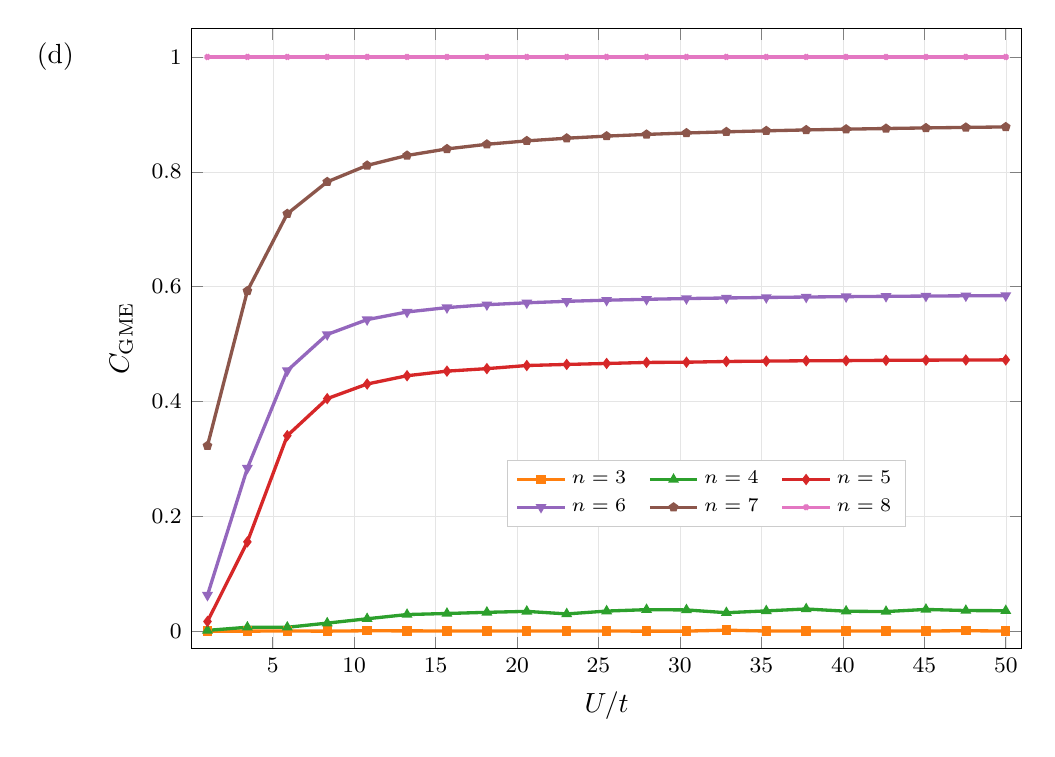
\begin{tikzpicture}
  \begin{axis}[
    width=\columnwidth,
    height=0.78\columnwidth,
    xlabel={$U/t$},
    ylabel={$C_{\mathrm{GME}}$},
    grid=both,
    grid style={line width=.1pt, draw=gray!20},
    tick label style={font=\footnotesize\rmfamily, /pgf/number format/fixed},
    label style={font=\normalsize\rmfamily},
    scaled ticks=false,
    legend style={font=\scriptsize\rmfamily, draw=gray!40, at={(0.5,1.03)}, anchor=south, /tikz/every even column/.append style={column sep=6pt}},
    legend cell align={left},
    legend columns=3,
    ymin=-0.03,
    ymax=1.05,
    xmin=0.02,
    xmax=50.98,
    legend style={at={(0.620,0.250)}, anchor=center, fill=white},
    after end axis/.append code={\node[anchor=east, font=\normalsize\rmfamily] at (axis description cs:-0.13,0.954) {(d)};},
  ]
    \addplot[color=gmeC1, mark=square*, mark size=1.1pt, line width=1.2pt] coordinates {
        (1,0.000027) (3.45,0.00008) (5.9,0.000279) (8.35,0.000053)
        (10.8,0.000729) (13.25,0.000484) (15.7,0.000416) (18.15,0.000175)
        (20.6,0.000142) (23.05,0.00022) (25.5,0.000195) (27.95,0.000112)
        (30.4,0.00013) (32.85,0.001713) (35.3,0.000275) (37.75,0.000342)
        (40.2,0.000365) (42.65,0.000196) (45.1,0.000226) (47.55,0.000816)
        (50,0.000169)
    };
    \addlegendentry{$n=3$}
    \addplot[color=gmeC2, mark=triangle*, mark size=1.1pt, line width=1.2pt] coordinates {
        (1,0.001368) (3.45,0.006876) (5.9,0.006765) (8.35,0.014024)
        (10.8,0.021602) (13.25,0.028958) (15.7,0.030782) (18.15,0.032818)
        (20.6,0.034473) (23.05,0.030047) (25.5,0.035002) (27.95,0.037476)
        (30.4,0.036986) (32.85,0.032141) (35.3,0.035328) (37.75,0.038667)
        (40.2,0.034721) (42.65,0.034156) (45.1,0.037853) (47.55,0.035923)
        (50,0.035619)
    };
    \addlegendentry{$n=4$}
    \addplot[color=gmeC3, mark=diamond*, mark size=1.1pt, line width=1.2pt] coordinates {
        (1,0.016861) (3.45,0.155557) (5.9,0.340486) (8.35,0.404947)
        (10.8,0.430411) (13.25,0.444816) (15.7,0.452822) (18.15,0.457192)
        (20.6,0.46262) (23.05,0.46451) (25.5,0.466183) (27.95,0.467976)
        (30.4,0.468367) (32.85,0.469647) (35.3,0.470287) (37.75,0.470898)
        (40.2,0.471118) (42.65,0.471675) (45.1,0.47198) (47.55,0.472264)
        (50,0.472406)
    };
    \addlegendentry{$n=5$}
    \addplot[color=gmeC4, mark=triangle*, mark size=1.1pt, mark options={rotate=180}, line width=1.2pt] coordinates {
        (1,0.062695) (3.45,0.283926) (5.9,0.453837) (8.35,0.516697)
        (10.8,0.542561) (13.25,0.555869) (15.7,0.563483) (18.15,0.568535)
        (20.6,0.571851) (23.05,0.574409) (25.5,0.576376) (27.95,0.577922)
        (30.4,0.579235) (32.85,0.580236) (35.3,0.581111) (37.75,0.581903)
        (40.2,0.582545) (42.65,0.583098) (45.1,0.583588) (47.55,0.58403)
        (50,0.584425)
    };
    \addlegendentry{$n=6$}
    \addplot[color=gmeC5, mark=pentagon*, mark size=1.1pt, line width=1.2pt] coordinates {
        (1,0.322896) (3.45,0.592553) (5.9,0.726943) (8.35,0.782475)
        (10.8,0.811119) (13.25,0.828414) (15.7,0.839827) (18.15,0.847873)
        (20.6,0.85384) (23.05,0.858461) (25.5,0.862116) (27.95,0.865082)
        (30.4,0.867537) (32.85,0.869599) (35.3,0.871357) (37.75,0.872872)
        (40.2,0.87419) (42.65,0.875349) (45.1,0.876374) (47.55,0.877287)
        (50,0.878107)
    };
    \addlegendentry{$n=7$}
    \addplot[color=gmeC6, mark=x, mark size=1.1pt, line width=1.2pt] coordinates {
        (1,1) (3.45,1) (5.9,1) (8.35,1)
        (10.8,1) (13.25,1) (15.7,1) (18.15,1)
        (20.6,1) (23.05,1) (25.5,1) (27.95,1)
        (30.4,1) (32.85,1) (35.3,1) (37.75,1)
        (40.2,1) (42.65,1) (45.1,1) (47.55,1)
        (50,1)
    };
    \addlegendentry{$n=8$}
  \end{axis}
\end{tikzpicture}
